\documentclass{article}

\usepackage{graphicx,hyperref,amsmath,natbib,bm,url}
\usepackage{float}
\usepackage{microtype, todonotes}
\usepackage[a4paper, text = {16.5 cm, 25.2 cm}, centering]{geometry}
\usepackage[compact, small]{titlesec}
\setlength{\parskip}{1.2ex}
\setlength{\parindent}{0em}
\clubpenalty = 10000
\widowpenalty = 10000



\begin{document}

\section{Photons}

\begin{enumerate}
    
    \item
	Directly ionizing radiation: Fast particles having a charge that transfers energy through a series of small Coulomb interactions.
    \item
	Indirectly ionizing radiation: Photons or neutrons which transfer energy to charged particles in the matter.

\end{enumerate}

The "cross section" is proportinonal with the interaction strenght.
A simple visulisation could be imagining two disks of radiis $r$, the total area is then 

\begin{equation}
    s = \pi (r_1^2 + r_2^2)
\end{equation}

Consider now $N$ particles coming towards an area $S$ with $n$ atoms.
The probability for interaction then becomes 

\begin{equation}
    p = \frac{n*\sigma}{S}
\end{equation}

and the with the number of \emph{interacting} particles

\begin{equation}
    Np = N\frac{n*\sigma}{S}
\end{equation}

We separate between electronic and atomic cross sections.
The cross sections depends on the type of target, and the type of the incoming particle.

The differential cross section is the number of particles scattered into the angle d$\Omega$ per units area.
For photons we can have (in principle) two different kinds of processes:

\begin{enumerate}

    \item
	Absorbtion
    \item
	Scattering
\end{enumerate}

\subsection{Scattering, Thompsom and Comton}

The scattering can be coherent, or incoherent. 

The coherent scattering is called Rayleigh scattering. Here the photon is scattered without loss of energy

The atomic cross section for Rayleigh-scattering is 

\begin{equation}
    \sigma_r \propto \left( \frac{Z}{h\upsilon} \right)^2
\end{equation}

Dependence mainly on atomic structire and photon energy. 
Larger $Z$ and smaller $h\upsilon$ will increase the chance for Rayleigh scattering

The incoherent scattering is called Comtpon-scattering.
Here, the photon will hit an electron (which can be considered almost free) and loose some energy.

We can simply consider the kinematics of what is happening and get the result:

\begin{equation}
    h\upsilon = \frac{h\upsilon}{1 + \frac{h\upsilon}{m_e c^2}(1 - \mathrm{cos} \theta)}
\end{equation}

The forward-scattered photons will have the same energy as the incoming photons, whereas the scattered photons of other angles will have lower and lower energy.
The cross section of Compton-scattering was derived by Klein and Nishina, with a free electron assumed

\begin{equation}
    \left( \frac{\mathrm{d}\sigma}{\mathrm{d}\theta} \right ) = \pi r_0^2 \left( \frac{\upsilon'}{\upsilon} \right)^2 \left( \frac{\upsilon'}{\upsilon} + \frac{\upsilon}{\upsilon'} - \mathrm{sin}^2\theta \right ) \mathrm{sin} \theta
\end{equation}

We can perform some substitution to get the cross section for a certain scatter-energy 

\begin{equation}
    \frac{\mathrm{d}\sigma}{\mathrm{d} ( h\upsilon')} = \frac{\pi r_0^2 m_e c^2}{(h \upsilon)^2} \left ( \frac{h\upsilon'}{h\upsilon} + \frac{h\upsilon}{h\upsilon'} -1 + \left ( 1  - \left( \frac{h\upsilon}{h\upsilon'} -1 \right ) \frac{m_e c^2}{h\upsilon} \right ) ^2 \right )
\end{equation}

The fractional cross section with respect to the scattered energy has a sharp rise at the lower limit, this is because the back-scattered photons can only have a certain energy.
At the upper max we could have a compton-edge, a rise of the cross section before an abrupt stop while we approach the incoming energy.

\begin{figure}
    \centering
    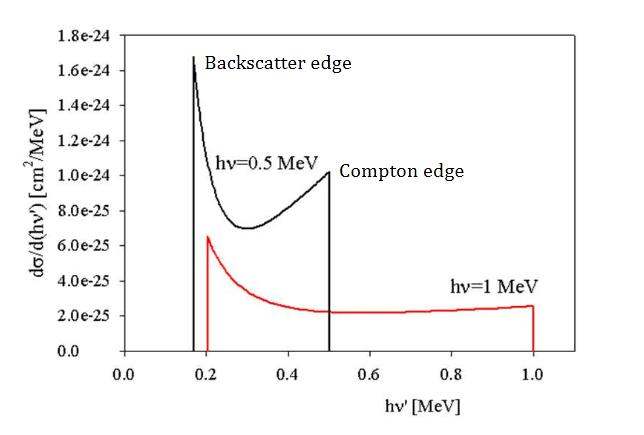
\includegraphics[width = 0.48\textwidth]{photons/figs/kleinnishinaenergy}
    \caption{Fractional cross section as a function of energy of the scattered photon}
\end{figure}

The Klein-Nishina cross section assumes a "free" electron, and for atomic electrons and for lower photon energies, this do not hold.
The cross section then becomes smaller for high $Z$-materials for lower energies.

In the compton process, some energy gets transfered to the electron:

\begin{equation}
    T = h\upsilon - h \upsilon'
\end{equation}

This energy transfer can be expressed as a fractional cross section, and gives a nice expression for the mean transfered energy

\begin{equation}
    \bar{T} = \frac{\sigma_{tr}}{\sigma} h \upsilon
\end{equation}

\subsection{Photo-electric effect}

A photon is absorbed by an atom or molecule, it can result in an excitation or an ionization.
An electron is ejected from the atom.
When the atom de-excites, it can give off characteristic radiation.

The energies of the atomic cross section depends on the atomic structure and the transition energies.
The probability for the emission is called flourecence yield.

A loosely bound electron gets ejected in the so-called Auger-effect.
The energy of the electron equals to the deexcitation of the atom. 
This effect dominates at low Z-materials. 
For high Z-materials, the dominant effect is characteristic radiation.

Hence, these two effects are competing de-excitation modes for the atom after a photon is absorbed.

The cross-section for the photo electric effect depends highly on the Z-number.
It is also inversely propotional to the photon energy.

\subsection{Pair production}

The photon gets absorbed in the nuclear electromagnietic field where it gets turned into an electron-positron pair. 
If it happens in the electromagnetic field of the electron, it is called triplet production.
The primary electron also receives some energy.

There is a nice summary of the interactions on slide 22 where the cross sections and the energies where the different effects are dominant are listed.


\subsection{Attenuation}

When the photons enters a material, they get attenuated. 
This attenuation, if we consider photons of the same energy and the same angle of incidence, follows a nice exponential drop-off of intensity.
It has to be stressed that this is only the "primary" photons, the do not neccecary get absorbed but could also simply change direction.
The coefficient of which this exponential follows can be expressed as the attenuation coefficient $\mu$ and the mass densitt $\rho$.
It is important to note that it is highly energy dependent.
There is also a coefficient of energy transfer.

Further more, for certain energies the ratio of the attenuation coefficients between for example soft tissue and bone is highly different. This is called the diagnostic window as it allows separation of soft tissue and bone in imaging.

Highly important to note that it is the probability of interaction, not absorbtion. 
To illustrate, we could think of an experiment where we meassure a narrow beam, and only count the phtons that have not scattered or are absorbed.

We can calculate the mean free path for the most likely value of the distribution of path-lenghts.
This lenght is the inverse of the mass attenuation coefficient.

\section{Charged particles}

For a charged particle, things look a bit different.
An incoming charged particle interacts with an atom or molecule, either it just exchange some energy and merely excites the atom, or it removes an electron and the result is an ionization.

One can derive from simple classical mechanics the crude estimate of the cross section of the electron.
This will not be covered here but some results:

\begin{enumerate}

	\item


		
\end{enumerate}







\section{Neutrons}

\section{Quantities}

\end{document}
